\newpage
\section{142. 环形链表 II}
\label{leetcode:142}

\subsection{题目}

给定一个链表,返回链表开始入环的第一个节点。 如果链表无环,则返回 null。

为了表示给定链表中的环,我们使用整数 pos 来表示链表尾连接到链表中的
位置(索引从 0 开始)。 如果 pos 是 -1,则在该链表中没有环。

\textbf{说明}:不允许修改给定的链表。

\textbf{示例 1}:

\begin{verbatim}
  输入:head = [3,2,0,-4], pos = 1
  输出:tail connects to node index 1
  解释:链表中有一个环,其尾部连接到第二个节点。
\end{verbatim}

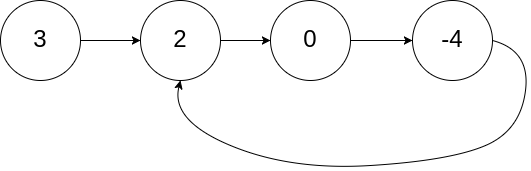
\includegraphics[width=100mm,height=50mm]{images/leetcode/circularlinkedlist.png}

\textbf{示例 2}:

\begin{verbatim}
  输入:head = [1,2], pos = 0
  输出:tail connects to node index 0
  解释:链表中有一个环,其尾部连接到第一个节点。
\end{verbatim}

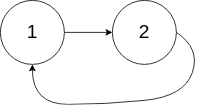
\includegraphics[width=60mm,height=30mm]{images/leetcode/circularlinkedlist_test2.png}

\textbf{示例 3}:

\begin{verbatim}
  输入:head = [1], pos = -1
  输出:no cycle
  解释:链表中没有环。
\end{verbatim}

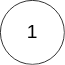
\includegraphics[width=15mm,height=15mm]{images/leetcode/circularlinkedlist_test3.png}

\textbf{进阶}:\\
你是否可以不用额外空间解决此题?

\subsection{参考题解}

\begin{verbatim}
/**
 * Definition for singly-linked list.
 * function ListNode(val) {
 *     this.val = val;
 *     this.next = null;
 * }
 */
/**
 * @param {ListNode} head
 * @return {ListNode}
 */
var detectCycle = function(head) {
  let ptr1 = getIntersection(head);
  if (ptr1 === null) {
    return null;
  }
  let ptr2 = head;

  while (ptr1 !== ptr2) {
    ptr1 = ptr1.next;
    ptr2 = ptr2.next;
  }
  return ptr1;
};

var getIntersection = function(head) {
  let slow = head;
  let fast = head;
  while (slow && fast && fast.next) {
    slow = slow.next;
    fast = fast.next.next;
    if (slow === fast) {
      return slow;
    }
  }
  return null;
};
\end{verbatim}
